\subsection{Regularization in DNNs (Exercise 6.3) \\ Problems + Solutions}
\textbf{Dying ReLu Problem:} Once a value becomes negative, it will always output 0. Since the gradient for neg. values is 0 in ReLu, it will not become active again. 
\begin{itemize}
	\item[$\Rightarrow$]\textit{ELU or leaky ReLU activation function that has a non-zero gradient for arguments smaller than zero.}
	$$
	\mathit{ELU}_\alpha = 
		\begin{cases}
			\alpha(\exp(z) - 1) & z< 0 \\
			z 					& z\geq 0
		\end{cases}
	$$
	\textit{with hyperparamter $\alpha$}.
\end{itemize}



\textbf{Slow learning of a DNN with sigmoid function using Gradient Descent algorithm and large initialized weights:} ) The sigmoid function saturates quickly and hence, for large values of $z$ the gradient updates are very small, slowing down the learning process.
\textit{\begin{itemize}
	\item[$\Rightarrow$] Use random initialization weights 
	\item[$\Rightarrow$] Apply different activation function( such as ReLU or its variations), that is nonsaturating for positive values
\end{itemize}
}


\textbf{Applying dropout layers to avoid overfitting: } This will increase the training time, since parameter updates become noisy due to omitting units in each training iteration.  \\
Inference time is not influenced, since dropout is only applied during training

\subsection{Variational Autoencoders (Notes 11)}
\textit{Learn meaningful representations without supervision.
}\begin{center}
\textbf{Representation Learning: }
	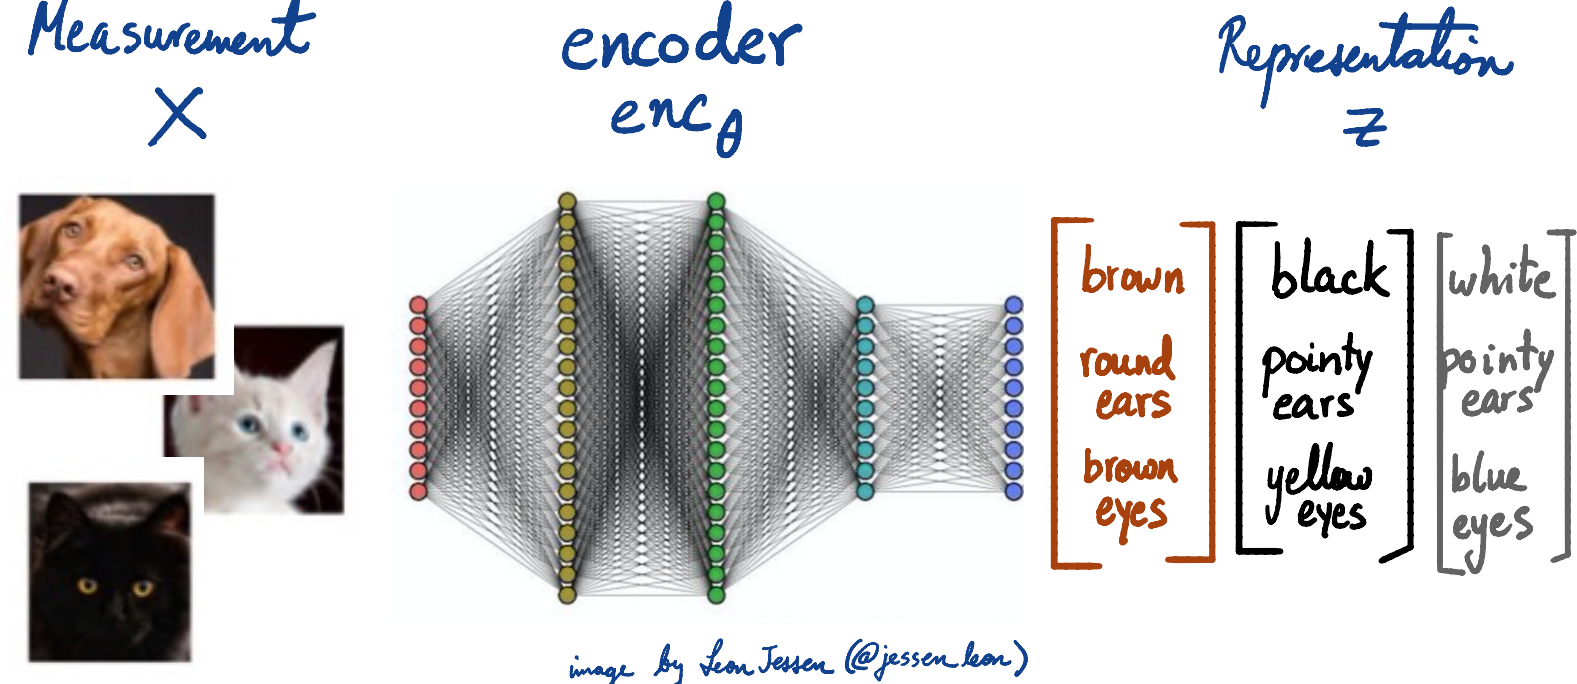
\includegraphics[width=0.8\columnwidth]{images/11-representation-learning}
\end{center}

\subsubsection{Objective}
Derive parametrized function $\enc_\theta$ that maps measurements in $\mathcal X$ to probability distributions over a representation space $\mathcal Z$
$$
	\enc_\theta: x \in \mathcal X \mapsto p_\theta(\cdot| x) \textit{ over } \mathcal Z 
$$


\textbf{Requirements for Autoencoder:}
\begin{itemize}
	\item Informative: Given representation, it should be easy to guess the measurement
	\item Disentangled: Every component in the representation is associated with a distinguished feature
	\item Robust: Noisy perturbations in the measurement should not substantially affect the representation and vice versa
\end{itemize}

\subsubsection{The info max principle (Linsker 1988)}
$Z = \enc_\theta(X)$ maximizes $I(X;Z)$

Information $(X;Z)$ is defined as
$$
	I(X;Z) = \E_{X,Z}\left[\log\left(\frac{p(X,Z)}{p(X)p(Z)} \right) \right]
$$
\begin{center}
	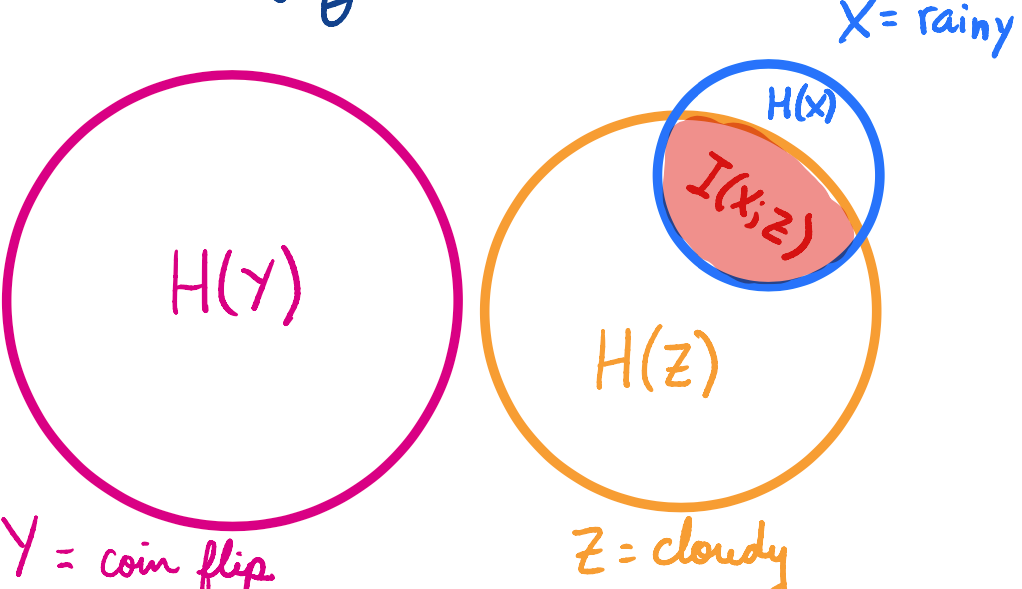
\includegraphics[width=0.5\columnwidth]{images/11-infomax-principle}
	$$
		H(x) = \E_x\left[-\log p(x)] \right]
	$$
\end{center}


\begin{minipage}{\columnwidth}
\textbf{Formalization}\\
Let $X$ and $Z$ be a measurement and a representation space. Let $F=\{\enc_\theta: \theta \in \Theta \}$ be a parametric family of functions with $\enc_\theta$ mapping $X$ to distributions over $Z$.

The encoder function $\enc_{\theta^*}$ is defined by 
$$
	\theta^* = \arg\max_\theta I(X; Z)
$$
where $Z$ is a random variable with distribution $\enc_\theta(X)$

This is informative, but not disentangled or robust. If $\enc_\theta$ is complex enough then $\enc_\theta$ maximizes $I(X;z)$ becoming an injective function from $X$ to $Z$.
	
\end{minipage}



\subsubsection{Variational Autoencoders (VAE)}
\textit{A VAE fits a generative probabilistic model to the dataset, where the representations are latent variables.}

\begin{minipage}{0.3\columnwidth}
	\begin{center}
		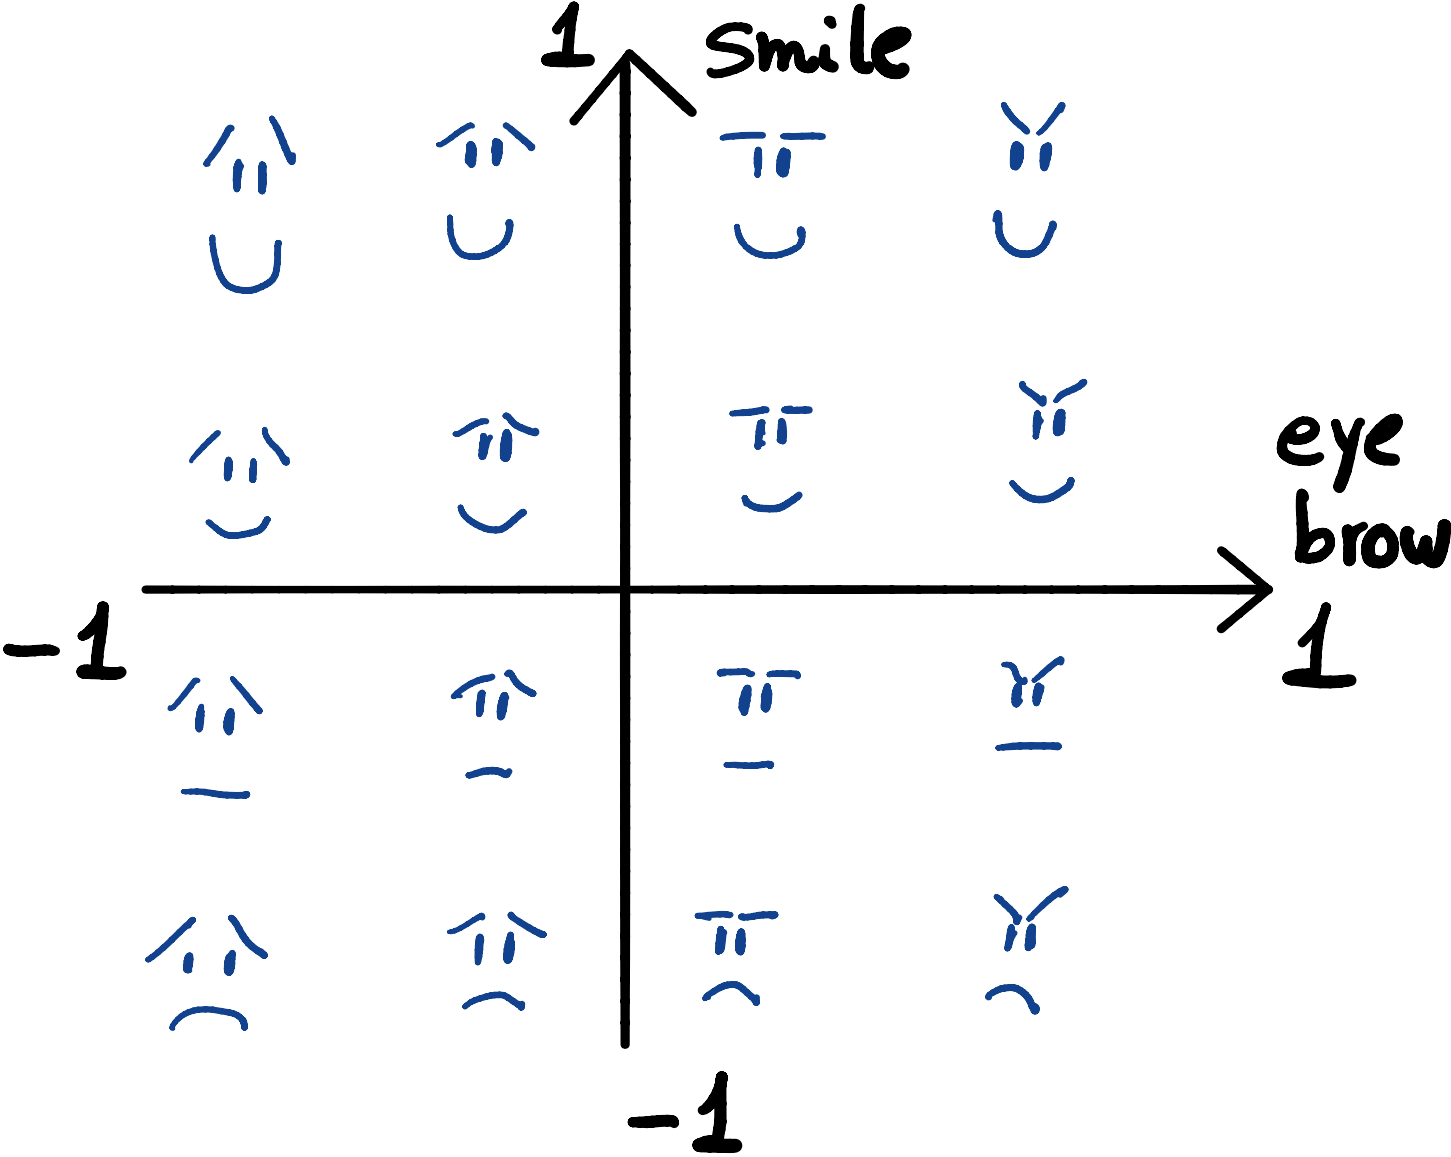
\includegraphics[width=\columnwidth]{images/11-autoencoders}
	\end{center}
\end{minipage}
\begin{minipage}{0.6\columnwidth}
\textbf{Smileys Example}
	\begin{itemize}
	\item Disentangled: $Z_0, Z_1$ along axes; in either direction only the smile OR the eye brows change
	\item Diagonal lines would be entangled.
\end{itemize}
\end{minipage}

\href{https://towardsdatascience.com/understanding-variational-autoencoders-vaes-f70510919f73}{Blogpost Link}

\textbf{Autoencoders: }
\begin{itemize}
	\item General Idea: Set an encoder and a decoder as neural networks and to learn the best encoding-decoding scheme using an iterative optimization process.
	\item At each iteration, compare encoded-decoded to initial data.
\end{itemize}



\textbf{Variational Autoencoders: }
\textit{Pick a family of distributions over the latent variables with its own variational parameters $q(z_{1:m}| \mathcal V)$. Then find the parameters that makes $q$ close to the desired posterior and use $q$ with the fitted parameters as a proxy for the posterior.} \href{https://www.cs.princeton.edu/courses/archive/fall11/cos597C/lectures/variational-inference-i.pdf}{(Princeton Advanced Methods in Probabilistic Modeling)}.

\begin{itemize}
	\item General Idea: autoencoder whose training is regularized to avoid overfitting and ensure that the latent space has good properties that enable generative process
	\item Autoencoders train encoder-decoder, but there is no way \textbf{generating new data}
	\item instead of encoding an input as a single point, encode it as a distribution over the latent space.
	\item In order to use an autoencoder for content generation, we have to make sure the distribution is regular (e.g. by using regularization terms).
\end{itemize}

\textbf{Variational Inference: } The process of finding an approximate posterior.
\begin{enumerate}
	\item Define prior and calculate likelihood (decoder)
	\item Find approximate posterior (encoder)
\end{enumerate}

\begin{highlight}{Variational Autoencoders}
\begin{enumerate}
	\item Define 
	\begin{itemize}
		\item $\{p_\theta'(z): \theta'\in \Theta'\}$ pram. family of priors
		\item $\{p_\theta(x|z): \theta\in \Theta\}$ pram. family of likelihoods
		\item $\{q_\phi(z): \phi\in \Phi'\}$ pram. f. of approx. posteriors
	\end{itemize}
	\item The variational auto encoder is trained by solving 
	$$
		\max_{\theta', \theta, \phi}\log p_{\theta', \theta, \phi}(x_1, ..., x_n), \{x_1, ..., x_n\} \textit{ training set}
	$$
	\item The representation $Z$ of a measurement $x$ is a random variable with pdf $q_\phi(z|x)$.\\ The measurement $X$ encoded by a representation $Z$ is a random variable with pdf $p_\theta(x|z)$
\end{enumerate}
\end{highlight}


\textbf{How to train a variational autoencoder? }
$$
	\arg\max_{\theta', \theta, \phi} \sumin \log p_{\theta', \theta}(x_i)
$$
{\footnotesize
\begin{align*}
	\log_{\theta', \theta}p(x_i) 	&= \E_{Z\sim q_\phi(\cdot| x_i)}\left[\log p_{\theta', \theta}(x_i)\right] \\
									&= \E_{Z\sim q_\phi(\cdot| x_i)}\left[\log \left(\frac{p_{\theta', \theta}(x_i, Z)}{p_{\theta'. \theta}(Z| x_i)}\frac{q_\phi(Z| x_i)}{q_\phi(Z| x_i)} \right)\right] \\
									&= \underbrace{\E_{Z\sim q_\phi(\cdot| x_i)}\left[\log \left(\frac{p_{\theta', \theta}(x_i, Z)}{q_\phi(Z| x_i)} \right)\right]}_{\mathit{elbo}_{\theta', \theta, \phi}(x_i)} \\
									&\quad\quad\quad  + \underbrace{E_{Z\sim q_\phi(\cdot| x_i)}\left[\log \left(\frac{q_\phi(Z| x_i)}{p_{\theta', \theta}(Z| x_i)} \right)\right] }_{\mathit{KL}\left(q_\phi(\cdot| x_i)\| p_{\theta', \theta}(\cdot| x_i)\right) \geq 0} \\
	\implies \log_{\theta', \theta}p(x_i) 
									&\geq \mathit{elbo}_{\theta', \theta, \phi}(x_i) \\
									&= \underbrace{\E_{Z\sim q_\phi(\cdot| x_i)}\left[\log \left(p_\theta(x_i| Z\right)\right]}_{\mathit{Infomax!}} \\
									&\quad\quad\quad  + \underbrace{E_{Z\sim q_\phi(\cdot| x_i)}\left[\log 
											\left(\frac{p_{\theta'}(Z)}{q_{\phi}(Z| x_i)} \right)\right] }_{\underbrace{\mathit{-KL}\left(q_\phi(\cdot| x_i)\| p_{\theta', \theta}(\cdot)\right) }_{\mathit{Regularization Term}}}  
\end{align*}
}
This is informative, disentangled and robust by the choice of $p_\theta(\cdot | Z)$ and $q_\phi(\cdot | x)$.
\subsubsection{Kullback-Leibler Divergence $\mathit{KL}$}
Used to measure the closeness of 2 distributions. Usually one of them is the approximation for the other. In our case: $q$ and $p$.
$$
	\mathit{KL}(q\|p) = \E_q\left[\log\frac{q(Z)}{p(Z|x)} \right]
$$
\subsubsection{The evidence lower bound $\mathit{elbo}$}
\textit{We can't minimize the KL divergence exactly. But we can minimize a function that is equal to it up to a constant: The $\mathit{elbo}$-function}

\textbf{The elbo is optimized using}
\begin{itemize}
	\item Gradient Descent
	\item Monte-Carlo Sampling
	\item Analytical Reparametrization tricks
\end{itemize}


\subsubsection{Denoising an Autoencoder}
Blank out parts of the input image during training to create a more robust encoder.

\subsubsection{Modeling Invariances}
If we want the autoencoder to be robust against rotations or scaling:
\begin{itemize}
	\item[$\Rightarrow$] Augmentation of training set
	\item[$\Rightarrow$] Special preprocessing of images
	\item[$\Rightarrow$] Implementation of invariances into multi-layer perceptrons (CNN) 
\end{itemize}

\subsection{Deep Generative Modeling}
We want to use generative modeling with DNN.


\subsubsection{Generative Adversarial Networks (GANs)}
\textit{Approach to generative modeling using deep learning methods (e.g. convolutional neural networks). In contrast to VAE, we do not model the density, but instead directly define a \textbf{sampler}.}\\
\textit{(Not covered in exam)}

\subsubsection{VAEs vs. GANs}
\begin{tabular}{ p{0.45\columnwidth} | p{0.45\columnwidth} }
		\textbf{VAE} & \textbf{GAN}\\\hline
  		\textbf{Pros: }
  		\begin{itemize}[leftmargin=*]
  			\item Principled approach
  			\item Allows inference of the encoder which might be useful for other tasks
  		\end{itemize}
  		& 
  		\textbf{Pros: }
  		\begin{itemize}[leftmargin=*]
  			\item Beautiful
  			\item State of the Art
  		\end{itemize}
  		\\\hline

  		\textbf{Cons: }
  		\begin{itemize}[leftmargin=*]
  			\item Maximizes the lower bound of the likelihood (quality is not as good, blurry)
  		\end{itemize}
  		&
  		\textbf{Cons: }
  		\begin{itemize}[leftmargin=*]
  			\item Tricky, unstable training
  			\item mode collapse
  			\item cannot solve inference queries as $p(x)$
  		\end{itemize} \\\hline
\end{tabular}

